\documentclass[a4paper,twoside,12pt,DIV=13,BCOR=5mm,numbers=noenddot,cleardoublepage=empty]{scrbook}
%======= Einbinden der benötigten Packete (= Zusatzfunktionen)
\usepackage[T1]{fontenc}                % für Fonts in westeuropäischer Codierung
\usepackage{lmodern}										% Latin Modern Paket verändert die verwendete Schriftart. Bessere Darstellung für pdf
\usepackage{textcomp}										% Provides extra symbols, e.g. arrows like \textrightarrow, various currencies (\texteuro,..
\usepackage[latin1]{inputenc}    				% german special characters
\usepackage[english,ngerman]{babel}     % hyphenation   usepackage[english,ngerman]{babel} f. deutsch
\usepackage{pdfpages}										% Einbinden von pdf-Files
\usepackage{pifont,textcomp,mathcomp}   % dingbad psfonts and text-compilant fonts (euro, TM, ...)
\usepackage{amsmath,amsopn,amsthm}      % AMS mathematics
\usepackage{amssymb}                    % zusätzliche Symbole 
\usepackage{xspace}											% avoids eaten spaces

%======= Eine Umgebung für Bilder und Tabellen			  	
%\usepackage[textfont={Small},labelfont={bf},margin=1cm,format=plain,font=singlespacing]{caption}   % hanging caption text [hang]
\usepackage[textfont={small},labelfont={bf},margin=1cm,format=plain,font=singlespacing]{caption}   % hanging caption text [hang]
\captionsetup*[figure]{name=Abb.}			 % Abbildungsunterschrift beginnt mit Abb.
\captionsetup*[table]{name=Tab.}


%======= Farben für Überschriften
\usepackage{color}
\definecolor{TUBlau}{rgb}{0,0.4,0.6}   % TU-blau RGB 0 102 153
\addtokomafont{sectioning}{\sffamily\bfseries\selectfont\color{TUBlau}}
\setkomafont{chapter}{\normalfont\huge\sffamily\bfseries\color{TUBlau}}
\addtokomafont{section}{\Large}
\addtokomafont{subsection}{\normalfont\Large\sffamily\bfseries\color{TUBlau}}
\addtokomafont{subsubsection}{\normalfont\large\sffamily\bfseries\color{TUBlau}}
\addtokomafont{paragraph}{\normalfont\large\sffamily\bfseries\color{TUBlau}}


%======= Kopf-/Fußzeilen
\pagestyle{plain} % nur Fußzeile



%======= Eine kompakte Umgebung für die Bilder
\newcommand{\bild}[4]{{
\begin{figure}[#2]
\begin{center}
\includegraphics[scale=#3]{pictures/#1}
\caption{#4}\label{fig:#1}
\end{center}
\end{figure}
}}


%======= Definitionen eigener Befehle
\newcommand{\degC}{\ensuremath{^{\circ}}C}        % Grad Celsius
\newcommand{\Gu}{\glqq{}}                         % Gänsefüßchen unten
\newcommand{\Go}{\grqq{}\xspace}    												% Gänsefüßchen oben











 
\usepackage{graphicx}
\usepackage{esvect}
\usepackage{bm}
\usepackage{mathtools}
\begin{document}
    \renewcommand{\baselinestretch}{1.25}
    \newcommand{\StudentA}{Philipp Hanser}
    \newcommand{\MatrNrA}{11775264}
    \newcommand{\StudentB}{Florian Strebl}
    \newcommand{\MatrNrB}{11712190}
    \newcommand{\StudentC}{Alexander Seiler}
    \newcommand{\MatrNrC}{11771276}

    \newcommand{\LUDatum}{06.06.2019}
    \newcommand{\LUGruppe}{Gr. 15}
    \newcommand{\LUBetreuer}{Geiginger, Lisa-Marie}  

    \large
    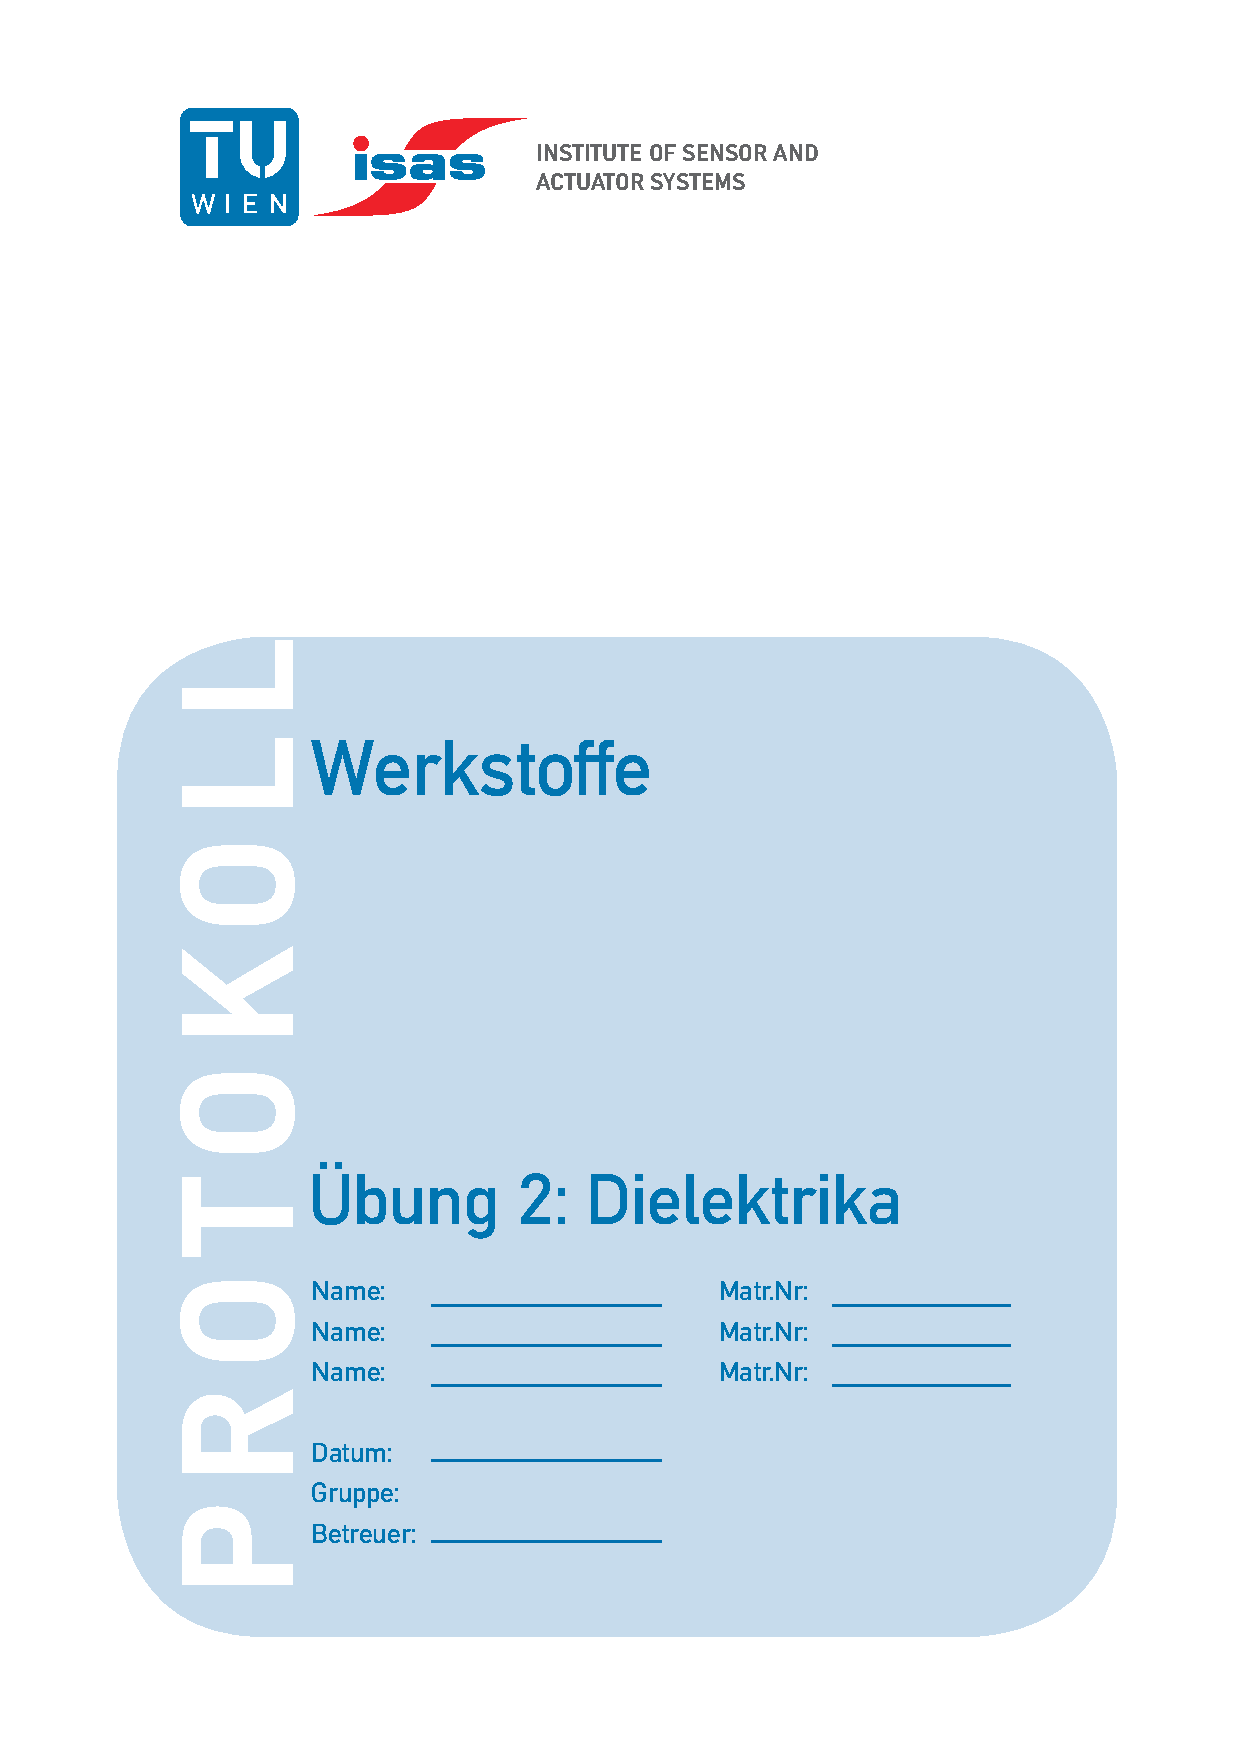
\includepdf[fitpaper=true,
                            picturecommand*={\unitlength1cm 
                            \put(7.3,7.7){\StudentA} \put(14.1,7.7){\MatrNrA}
                \put(7.3,7.0){\StudentB} \put(14.1,7.0){\MatrNrB}
                \put(7.3,6.3){\StudentC} \put(14.1,6.3){\MatrNrC}
                            \put(7.3,5.1){\LUDatum} 
                \put(7.3,4.4){\LUGruppe} 
                \put(7.3,3.7){\LUBetreuer} 
    }]
    {pictures/DeckblattLUDie}


    \setcounter{tocdepth}{3}

    \setcounter{page}{0}
    \renewcommand{\thepage}{\roman{page}}
    \tableofcontents \cleardoublepage

    \setcounter{page}{1}
    \renewcommand{\thepage}{\arabic{page}}
    \setcounter{chapter}{0}

    \chapter{Durchgangs- und Oberfl\"achenwiderstand}
        \section{Grundlagen}
            \subsection{Durchgangswiderstand}
            \subsection{Oberfl\"achenwiderstand}
        \section{Aufgabenstellung}
        Im Zuge des Dielektrika-Labors sollen f\"unf verschiedene Dielektrika 
        zum Messen herangezogen werden. Bei jedem dieser Dielektrika sollen 
        jeweils Durchgangswiderstand als auch Oberfl\"achenwiderstand gemessen 
        werden. Die f\"unf Dielektrika sind PVC, Phenolharz, Teflon, Plexiglas und 
        Epoxidharz\\
        Wichtig ist jedoch dass darauf geachtet wird das die Messwerte jeweils zum 
        gleichen Zeitpunkt nach dem Einschalten des Messger\"ates aufgenommen werden.
        In diesem Fall wird jeweils nach einer vollen Minute der Messwert 
        aufgenommen, um die Messwerte der unterschiedlichen Dielektrika vergleichen
        zu k\"onnen.
        \\
        \\
        Die Proben, die gemessen werden, werden jeweils zwischen zwei Elektroden
        mit einem Schutzring herum platziert (siehe Abbildung Abb.~\ref{fig:elektrodenanordnung_widerstand.PNG}).
        Die Messzelle wird dabei f\"ur beide Arten der Widerstandsmessung herangezogen,
        sie wird lediglich anders beschaltet.

        \bild{elektrodenanordnung_widerstand.PNG}{!h}{1}{Elektrodenanordnung der Messzelle}
        \section{Durchgangswiderstand}
            \subsection{\"Ubungsaufbau}
            Als Messgerät wird ein Ohmmeter MILLI-TO 2 der Frima Dr. Kamphause 
            verwendet. Der Widerstand wird darauf digital angezeigt 
            (Messbereich: 50m$\Omega$ - 200 T$\Omega$; Messgenauigkeit: $\pm$1,5\%,
            $\pm$1 Digit bei 23 $^{\circ}$C). Abbildung 
            Abb.~\ref{fig:elektrodenanordnung_widerstand.PNG} zeigt die Messzelle und deren Aufbau.
            \\
            \\
            \bild{messaufbau_durchgang.PNG}{t}{1}{Beschaltung der Messzelle zum Messen des Durchgangswiderstandes}
            Abbildung Abb.~\ref{fig:messaufbau_durchgang.PNG} zeigt die Schaltung zum 
            Aufnehmen des Durchgangswiderstandes. Wichtig dabei ist anzumerken, dass auch 
            der Schutzring angeschlossen ist. Dies ist notwendig, da das Dielektrikum nicht nur 
            einen Durchgangswiderstand sonder auch einen Oberfl\"achenwiderstand. Dieser 
            erm\"oglicht auch eine Ladungstr\"agerbewegung \"uber die Oberfl\"ache der Probe.
            Um diesen parasit\"aren Oberfl\"achenstrom abzufangen, wird der Schutzring 
            mitbeschaltet. So wandern die Ionen nicht zur Gegenelektrode, sondern \"uber den Schutzring.
            \subsection{Ergebnisse und Erkenntnisse}
            Die Messwerte wurden jeweils nach einer Minute im Betrieb aufgenommen.
            \begin{table}[h]
                \begin{center}
                    \begin{tabular}{|c||c|c|}
                        \hline
                        Material & $R_D$ in $\Omega$ & $\rho_D$ in $\Omega$m \\
                        \hline
                        \hline
                        Plexiglas & * & * \\
                        \hline
                        Phenolharz & * & * \\
                        \hline
                        PVC & * & * \\
                        \hline
                        Teflon & * & * \\
                        \hline
                        Epoxidharz & * & * \\
                        \hline
                    \end{tabular}
                    \caption{Ergebnisse der Messung und errechneter Durchgangswiderstand}
                    \label{tab:table1}
                \end{center}
            \end{table}
        \section{Oberfl\"achenwiderstand}
            \subsection{\"Ubungsaufbau}
            \subsection{Ergebnisse und Erkenntnisse}
    \chapter{Dieelektrizit\"atszahl}

    \chapter{Durchschlagsfestigkeit}
\end{document}